%==========================================================================
% DESIGN COMPONENTS
%==========================================================================
\section{Memory Map}
\label{sec:memmap}
%
%==========================================================================
% PROTECTION DOMAINS
%==========================================================================
%
\subsection{Protection Domains}
%
Our \textit{fault model} for memory protection is the corruption of state belonging to a module caused due to illegal write operations made by some another module.
%
We create and enforce \emph{Protection Domains} within data memory address space of the embedded processor.
%
Protection domain refers to a fragmented but logically distinct portion of overall data memory address space (Figure ~\ref{fig:prot_domains}).
%
Every module stores its state in its own protection domain.
%
No assumptions are made about layout of state within a domain.
%
Modules are restricted from writing to memory outside their domain through run-time checks.
%
There is one single trusted domain in the system that is allowed to access all memory.
%

Protection models based on domains do not address all possible memory corruption faults in the system.
%
Modules can still corrupt their own state as it resides completely within a protection domain. 
%
This form of corruption, though undesirable, is less serious than corruption across domains.
%
If we have an operating system we can load the kernel image in its separate domain.
%
A stable kernel can always ensure a clean re-start of user modules when corruption is detected.
%
\begin{figure}[htbp]
   \centering
   \includegraphics[height = 1in, keepaspectratio=true]{figures/domains.pdf} 
   \caption{Protection Domains}
   \label{fig:prot_domains}
\end{figure}
%
%========================================================================================================================================
% MEMORY MAP DATA STRUCTURE
%========================================================================================================================================
\subsection{Memory Map Data Structure}
%
%
Creating and enforcing protection domains is a challenging task on resource constrained embedded platforms.
%
Limited memory prohibits static contiguous partitioning of address space into multiple domains.
%
Instead we partition the address space of the microcontroller into blocks of equal sizes.
%
A \textit{Block} is a small contiguous region of memory.
%
Memory is allocated to domains as \textit{segments}, which are simply sets of contiguous blocks.
%
Allocation of segments to domains could be static (at compile time) or dynamic (through a memory heap).
%
A domain could be allocated multiple segments that are scattered randomly across entire address space.
%
\textit{The Memory Map contains access permissions for every block of address space.}
%
The Memory Map specifies two pieces of information.
% 
First, it contains ownership information (domain identity) for every block of memory.
%
Second, it encodes information about memory layout such as start of a logical segment of allocation to programs.
%
An example of actual encoded information and their meaning is specified in Table~\ref{tab:mmap_table}.
%
\begin{table}[htdp]
\centering
\small{
\begin{tabular}{|c|l|}
	\hline
	Code & Meaning\\
	\hline
	1111 & Free or Start of Trusted Segment\\
	1110 & Later portion of Trusted Segment\\
	xxx1 & Start of Domain (0 - 6) Segment \\
	xxx0 & Later portion of Domain (0 - 6) Segment\\
	\hline
\end{tabular}}
\caption{Encoded information in memory map table for multi-domain protection}
\label{tab:mmap_table}
\end{table}
%
%
%========================================================================================================================================
% MEMORY MAP CHECKER
%========================================================================================================================================
\subsection{Memory Map Checker}
%
A memory map checker is required to validate memory accesses made by software components.
%
It enforces the protection model that we described earlier; programs can write only into their domain.
%
The memory map checker is implemented as a functional unit (MMC) that intercepts the signals generated by the CPU for writing into the data memory (Figure~\ref{fig:mmcramcpu}).
%
If the write address is valid the MMC writes directly into the data memory.
%
\begin{figure}[htbp]
   \centering
   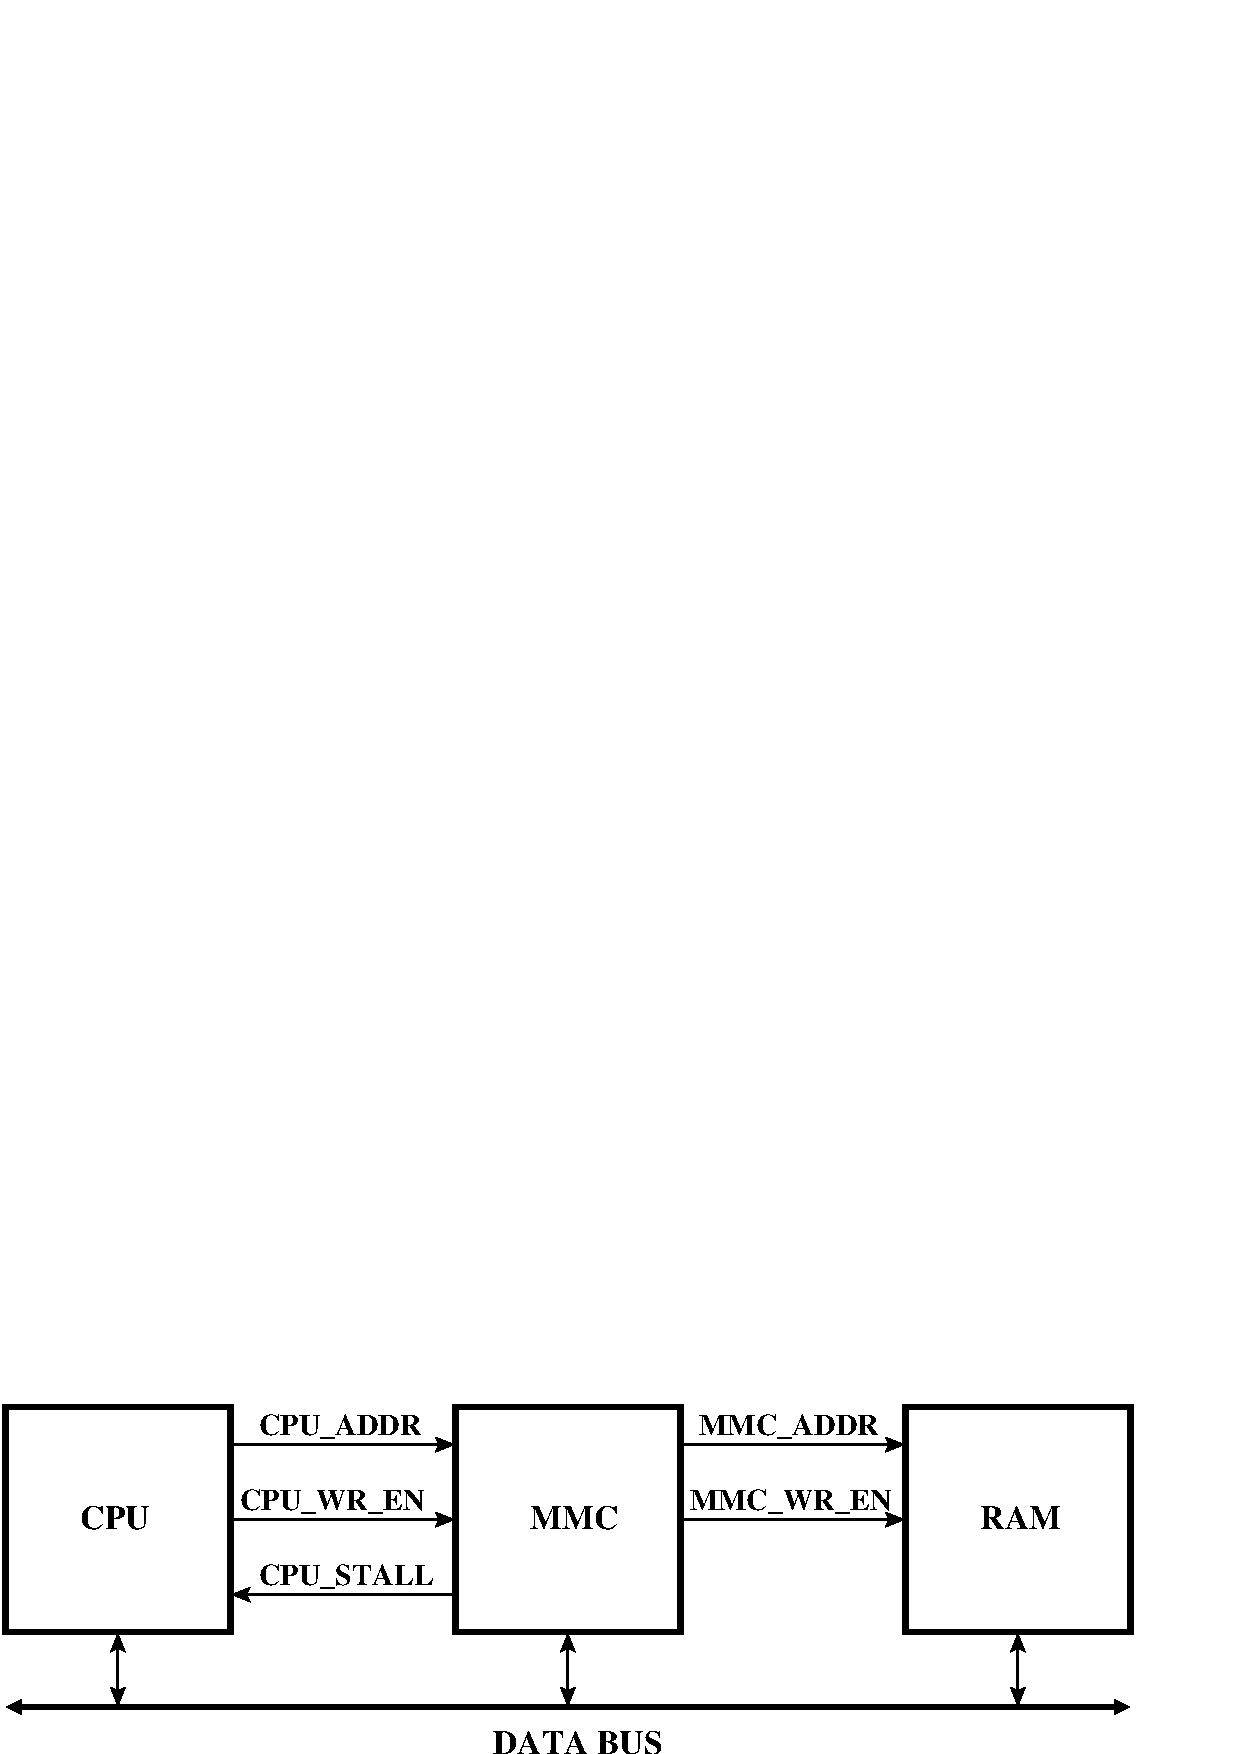
\includegraphics[height=0.5in, keepaspectratio=true]{figures/mmcramcpu.pdf} 
   \caption{Memory Map Controller (MMC)}
   \label{fig:mmcramcpu}
\end{figure}
%

The operations performed by MMC are three-fold.
%
First, it stalls the processor execution and takes control of the address bus to memory.
%
This occurs in the second cycle of the clock waveform shown in Figure~\ref{fig:mmcop}.
%
In the same clock cycle it performs an address translation operation to determine the address of the permissions in the memory map.
%
Address translation is shown in Figure~\ref{fig:memtrans}.
%
Memory map permissions are also read in this cycle as the MMC unit has control over the address bus.
%
Second, the MMC compares the ownership information to the identity of the current executing domain.
%
Finally, if the check is successful, then the MMC issues a write enable signal to the data memory.


The subset of address space protected by the memory map is defined by the register pair \texttt{mem\_prot\_bottom} and \texttt{mem\_prot\_top}.
%
The first step during translation is to determine the offset of the write address into the protected address space.
%
This is done by subtracting the lower bound of protected memory address space from the issued write address. 
%
Assuming a block size of 8 bytes, the nine significant bits of the address offset represent the block number.
%
Permissions are packed into a byte.
%
If the encoded information is stored in four bits (assuming multi-domain protection), then each byte would contain information of two contiguous memory blocks.
%
Therefore the last bit of the block number represents the byte offset of the permission.
%
The remaining bits index into the Memory Map Table.
%
The base pointer of the Memory Map Table is stored in a special register called \texttt{mem\_map\_base}.
%
The address of the permissions byte is computed by adding the memory map index to the memory map base pointer.
%
%
\begin{figure}[t]
  \centering
    \mbox{
      \subfigure[Timing]{\label{fig:mmcop}\includegraphics[height=1.2 in, keepaspectratio = true]{figures/mmcop.pdf}}\quad
      \subfigure[Addr Translate]{\label{fig:memtrans}\includegraphics[height = 1.25in, keepaspectratio = true]{figures/memaddrtrans.pdf}}
    }
    \caption{MMC Operations}
    \label{fig:mmc}
\end{figure}

%
%
The Memory Map data structure is configurable through a set of programmable registers shown in Table~\ref{tab:mmap_config}.
%
The registers are accessible only by the run-time library loaded in the trusted domain.
%
The \texttt{mem\_map\_config} register is used to configure the block size and the number of protection domains available in the system.
%
\begin{table}[htdp]
\centering
\small{
\begin{tabular}{|l|l|}
	\hline
	Register & Function\\
	\hline
	\texttt{mem\_map\_base} & Memory map base pointer \\
	\texttt{mem\_prot\_bot} & Lower bound of protected address space\\
	\texttt{mem\_prot\_top} & Upper bound of protected address space\\
	\texttt{mem\_map\_config} & Configure block size and domains\\
	\hline
\end{tabular}}
\caption{Memory Map Configuration Registers}
\label{tab:mmap_config}
\end{table}
%
%========================================================================================================================================
% MEMORY MAP SOFTWARE LIBRARY
%========================================================================================================================================
\subsection{Memory Map Software Library}
\label{subsec:mmap_for_protection}
%
The software library manages all the memory available on the embedded processor.
%
First, it ensures that the memory map accurately reflects current ownership and layout.
%
In any real system, memory is constantly allocated, de-allocated or transferred from one module to another.
%
The Memory Map should be immediately updated when any of these events occur.
%
The library provides \texttt{malloc}, \texttt{free} and \texttt{change\_own} calls that automatically update the  Memory Map data structure. 
%
Second, it only permits the  block owner to free or change its ownership.
%
This condition is necessary as one module may (due to programming errors) free up memory that is being used by other module in the system.
%
Also it prevents a module from accidentally hijacking memory that is owned by other modules.
%
To enforce this condition, the software library reads the identity of the current active domain from the status register.
%
%We describe implementation details of tracking current active application in Section~\ref{sec:cfmgr}.
%
Third, the software library sets up the memory map to be located in a protected region of memory.
%
This prevents accidental corruption of the Memory Map data structure.
%
It is the responsibility of the software library to ensure that a memory map of sufficient size is allocated in the system.
%
Fourth, it initializes the MMC with the appropriate block size, number of protection domains and the range of protected address space.
%





